\documentclass[10pt,a4paper]{article}
\usepackage[UTF8,fontset = windows]{ctex}
\setCJKmainfont[BoldFont=黑体,ItalicFont=楷体]{华文中宋}
\usepackage{amssymb,amsmath,amsfonts,amsthm,mathrsfs,dsfont,graphicx}
\usepackage{ifthen,indentfirst,enumerate,color,titletoc}
\usepackage{tikz}
\usepackage{multicol}
\usepackage{makecell}
\usepackage{longtable}
\usepackage{ifthen}
\usetikzlibrary{arrows,calc,intersections,patterns,decorations.pathreplacing,3d,angles,quotes}
\usepackage[bf,small,indentafter,pagestyles]{titlesec}
\usepackage[top=1in, bottom=1in,left=0.8in,right=0.8in]{geometry}
\renewcommand{\baselinestretch}{1.65}
\newtheorem{defi}{定义~}
\newtheorem{eg}{例~}
\newtheorem{ex}{~}
\newtheorem{rem}{注~}
\newtheorem{thm}{定理~}
\newtheorem{coro}{推论~}
\newtheorem{axiom}{公理~}
\newtheorem{prop}{性质~}
\newcommand{\blank}[1]{\underline{\hbox to #1pt{}}}
\newcommand{\bracket}[1]{(\hbox to #1pt{})}
\newcommand{\onech}[4]{\par\begin{tabular}{p{.9\textwidth}}
A.~#1\\
B.~#2\\
C.~#3\\
D.~#4
\end{tabular}}
\newcommand{\twoch}[4]{\par\begin{tabular}{p{.46\textwidth}p{.46\textwidth}}
A.~#1& B.~#2\\
C.~#3& D.~#4
\end{tabular}}
\newcommand{\vartwoch}[4]{\par\begin{tabular}{p{.46\textwidth}p{.46\textwidth}}
(1)~#1& (2)~#2\\
(3)~#3& (4)~#4
\end{tabular}}
\newcommand{\fourch}[4]{\par\begin{tabular}{p{.23\textwidth}p{.23\textwidth}p{.23\textwidth}p{.23\textwidth}}
A.~#1 &B.~#2& C.~#3& D.~#4
\end{tabular}}
\newcommand{\varfourch}[4]{\par\begin{tabular}{p{.23\textwidth}p{.23\textwidth}p{.23\textwidth}p{.23\textwidth}}
(1)~#1 &(2)~#2& (3)~#3& (4)~#4
\end{tabular}}
\begin{document}

\begin{enumerate}[1.]
\item 用列举法表示下列集合:\\
(1) $10$以内的所有素数组成的集合;\\
(2) $\{y|y=x-1,\  0\le x\le 3,\ x\in \mathbf{Z}\}$.
\item 用描述法表示下列集合:\\
(1) 被$3$除余$1$的所有自然数组成的集合;\\
(2) 比$1$大又比$10$小的所有实数组成的集合;\\
(3) 平面直角坐标系中坐标轴上所有点组成的集合.
\item 集合$\{(x, y)|xy>0, \ x,y\text{为实数}\}$是指\bracket{20}.
\twoch{第一象限内的所有点组成的集合}{第三象限内的所有点组成的集合}{第一象限和第三象限内的所有点组成的集合}{不在第二象限也不在第四象限内的所有点组成的集合}
\item 用符号``$\subset$''``$=$''或``$\supset$''连接集合$A$与$B$:\\
(1) $A=\{x|x^2-2x+1=0\}$, $B=\{x|x^2-1=0\}$;\\
(2) $A=\{1, 2, 4, 8\}$, $B=\{x|x$是$8$的正约数$\}$.
\item 已知集合$A=\{1\}$, $B=\{x|x^2-3x+a=0\}$. 是否存在实数$a$, 使得$A\subset B$?  若存在, 求$a$的值; 若不存在, 说明理由.
\item 已知集合$A=\{x, y\}$, $B=\{2x, 2x^2\}$, 且$A=B$. 求集合$A$.
\item 已知集合$A=\{x|x\le 7\}$, $B=\{x|x<2\}$, $C=\{x|x>5\}$. 求: $A\cap B$, $A\cap C$, $A\cap (B\cap C)$.
\item 已知集合$A=\{(x, y)|y=-x+1\}$, $B=\{(x, y)|y=x^2-1\}$. 求$A\cap B$.
\item 已知全集$U=\mathbf{R}$, 集合$A=\{x|4-x>2x+1\}$. 求$\overline A$.
\item 已知集合$A=\{2, (a+1)^2, a^2+3a+3\}$, 且$1\in A$. 求实数$a$的值.
\item 已知集合$A=\{x|x=2n+1,\ n\in \mathbf{Z}\}$, $B=\{x|x=4n-1,\ n\in \mathbf{Z}\}$. 判断集合$A$与$B$的包含关系, 并证明你的结论.
\item 设$a$是实数, 集合$M=\{x|x^2+x-6=0\}$, $N=\{y|ay+2=0\}$. 是否存在$a$, 使得$N\subset M$? 若存在, 求这些$a$的值; 若不存在, 说明理由.
\item 已知集合$A=\{1, 4, x\}$, $B=\{1, x^2\}$, 且$A\cup B=A$. 求$x$的值及集合$A$、$B$.
\item 判断下列语句是否为命题:\\
(1) 有的正方形是三角形;\\
(2) 任意一个三角形的内角和都为$180^\circ$;\\
(3) $1$是自然数吗?\\
(4) $3>\pi$;\\
(5) $2\in (0, 5)$, 且$2\in \mathbf{Z}$.
\item 判断下列命题的真假, 并说明理由:\\
(1) 如果$a$、$b$都是奇数, 那么$a+b$是偶数;\\
(2) 一组对边平行且两对角线等长的四边形是平行四边形;\\
(3) 如果$A\cap B=A$, 那么$A\cup B=B$.
\item 如果$a$、$b$、$c$为实数, 设$\alpha$: $a=b=c=0$; $\beta$: $a$、$b$、$c$中至少有一个为$0$; $\gamma$: $a^2+\sqrt b+|c|=0$. 那么$\alpha$\blank{20}$\beta$; $\alpha$\blank{20}$\gamma$; $\beta$ \blank{20}$\gamma$. (用符号``$\Leftarrow$''``$\Rightarrow$''或``$\Leftrightarrow$''填空)
\item 下列各组中, $\alpha$是$\beta$的什么条件?\\
(1) $\alpha$: 四边形$ABCD$的四条边等长, $\beta$: 四边形$ABCD$是正方形;\\
(2) $\alpha$: $\triangle ABC$与$\triangle DEF$全等, $\beta$: $\triangle ABC$与$\triangle DEF$的周长相等;\\
(3) $\alpha$: $x$是$2$的倍数, $\beta$: $x$是$6$的倍数;\\
(4) $\alpha$: 集合$A\subseteq B$, $B\subseteq C$, $C\subseteq A$, $\beta$: 集合$A=B=C$;\\
(5) $\alpha$: $A\cap B=A\cap C$, $\beta$: $B=C$.
\item 已知$l$、$m$都是自然数, 试判断``$l+m$是偶数''与``$l$、$m$都是偶数''是否等价, 并说明理由.
\item 证明: ``四边形$ABCD$是平行四边形''是``四边形$ABCD$的对角线互相平分''的充要条件.
\item 判断下列命题的真假, 并说明理由:\\
(1) 若$A\cap B=\varnothing$, $C\subset B$, 则$A\cap C=\varnothing$;\\
(2) 若$a$、$b\in \mathbf{R}$, 则关于$x$的方程$(a+1)x+b=0$的解为$x=- \dfrac b{a+1}$.
\item 已知$a$为实数. 写出关于$x$的方程$ax^2+2x+1=0$至少有一个实根的一个充要条件、一个充分非必要条件和一个必要非充分条件.
\item 若$\alpha$: $\{2\}\subset B\subseteq \{2, 3, 4\}$, $\beta$: $B=\{2, 4\}$, 则$\alpha$是$\beta$的\bracket{20}.
\twoch{充分非必要条件}{必要非充分条件}{充要条件}{既非充分又非必要条件}
\item 已知$\alpha$: $x<3m-1$或$x>-m$, $\beta$: $x<2$或$x\ge 4$.\\
(1) 若$\alpha$是$\beta$的充分条件, 求实数$m$的取值范围;\\
(2) 若$\alpha$是$\beta$的必要条件, 求实数$m$的取值范围. 
\item 设$a\in \mathbf{R}$, 求关于$x$的方程$ax=2$的解集.
\item 设$k\in \mathbf{R}$, 求关于$x$与$y$的二元一次方程组$\begin{cases}y=-2x+1,\\  y=kx-3\end{cases}$的解集.
\item 设$a\in \mathbf{R}$, 求一元二次方程$x^2-2ax+a^2-4=0$的解集.
\item 已知等式$2x^2+3x+5=a(2x+1)(x+1)+c$恒成立, 求常数$a$、$c$的值.
\item 已知一元二次方程$ax^2+bx+c=0$($a\ne 0$)的两实根为$x_1$、$x_2$, 求证: $|x_2-x_1| = \dfrac{\sqrt{b^2-4 ac}}{|a|}$.
\item 已知一元二次方程$x^2+3x-3=0$的两个实根分别为$x_1$、$x_2$, 求作二次项系数是$1$, 且分别以下列数值为根的一元二次方程:\\
(1) $-x_1, -x_2$;\\
(2) $2x_1+1, 2x_2+1$;\\
(3) $\dfrac 1{x_1}, \dfrac 1{x_2}$;\\
(4) $x_1^2, x_2^2$.
\item 设$a$、$b$、$c$、$d$为实数, 判断下列命题的真假:\\
(1) 若$a>b\ge 0$, 则$a^2>b^2$;\\
(2) 若$\sqrt a>\sqrt b$, 则$a>b$;\\
(3) 若$a>b>0, c>d>0$, 则$ac>bd$;\\
(4) 若$\dfrac ba>0$, 则$ab>0$;\\
(5) 若$a>b>0$, 则$a^2>ab>b^2$;\\
(6) 若$\sqrt a>b$, 则$a>b^2$.
\item 如果$a^2>b^2$, 那么下列不等式中成立的是\bracket{20}.
\fourch{$a>0>b$}{$a>b>0$}{$|a|>|b|$}{$a>|b|$}
\item 如果$a<b<0$, 那么下列不等式中成立的是\bracket{20}.
\fourch{$\dfrac ab<1$}{$a^2>ab$}{$\dfrac1{b^2}<\dfrac 1{a^2}$}{$\dfrac 1a<\dfrac 1b$}
\item 如果$a<0<b$, 那么下列不等式中成立的是\bracket{20}.
\fourch{$\sqrt{-a}<\sqrt{-b}$}{$a^2<b^2$}{$a^3<b^3$}{$ab>b^2$}
\item 证明: ``$a>0$且$b>0$''是``$a+b>0$且$ab>0$''的充要条件.
\item 设$x$是实数, 比较$(x+1)(x^2-x+1)$与$(x-1)(x^2+x+1)$的值的大小.
\item 试比较下列各数的大小, 并说明理由:\\
(1) $3+\sqrt 3$与$2+\sqrt 5$;\\
(2) $\sqrt 3+\sqrt 5$与$\sqrt 2+\sqrt 6$.
\item 设$a$、$b$为实数, 比较$a^2+b^2$与$2a-2b-2$的值的大小.
\item 已知$a>b$, $c>d$. 求证: $ac+bd>ad+bc$.
\item 已知$a\ge -1$, 求证$: a^3+1\ge a^2+a$.
\item 已知$a$、$b$为任意给定的正数, 求证: $a^3+b^3\ge ab^2+ba^2$, 并指出等号成立的条件.
\item 设$a$为实数, 求关于$x$的方程$2x+a^2=ax+4$的解集.
\item 设$m$为实数, 求关于$x$的方程$(m+1)x^2+6mx+9m=1$的解集.
\item 已知等式$2x^2-3x-1=a(x-1)^2+b(x-1)+c$恒成立, 其中$a$、$b$、$c$为常数. 求$a-b+c$的值.
\item 对一元二次方程$ax^2+bx+c=0$($a\ne 0$), 证明: $ac<0$是该方程有两个异号实根的充要条件.
\item 已知一元二次方程$2x^2+x-3=0$的两个实根分别为$x_1$、$x_2$, 求作二次项系数是$1$, 且分别以下列数值为根的一元二次方程:\\
(1) $x_1+x_2, x_1x_2$;\\
(2) $2x_1^2+1, 2x_2^2+1$;\\
(3) $\dfrac{x_2}{x_1}$, $\dfrac{x_1}{x_2}$;\\
(4) $x_1^4$, $x_2^4$.
\item 已知一元二次方程$x^2-2mx+m-1=0$的两实根为$x_1$、$x_2$, 且$x_1^2+x_2^2=4$. 求实数$m$的值.
\item 已知实数$a$、$b$、$c$满足$a+b+c=0$, 且$a>b>c$. 求证: $a>0$且$c<0$.
\item 设$s=a+b$, $p=ab$($a$、$b\in\mathbf{R}$), 写出``$a>1$且$b>1$''用$s$、$p$表示的一个充要条件, 并证明.
\item 原有酒精溶液$a$(单位: $\text{g}$), 其中含有酒精$b$(单位: $\text{g}$), 其酒精浓度为$\dfrac ba$. 为增加酒精浓度, 在原溶液中加入酒精$x$(单位: $\text{g}$), 新溶液的浓度变为$\dfrac{b+x}{a+x}$. 根据这一事实, 可提炼出如下关于不等式的命题:若$a>b>0$, $x>0$, 则$\dfrac ba<\dfrac{b+x}{a+x}<1$. 试加以证明. 
\item 解下列不等式(组):\\
(1) $2(x+1)-3(x-2)>8$;\\
(2) $\begin{cases} 3x-2(5-3x)>8,\\ 2x\le 2(2x+3). \end{cases}$
\item 解下列关于$x$的不等式:\\
(1) $ax+4<2x+a^2$, 其中$a>2$;\\
(2) $mx+1>x+m^3$, 其中$m<1$;\\
(3) $(p-q)x<p^2-q^2$, 其中$p\ne q$.
\item 解下列不等式:\\
(1) $(x-2)(3-x)\le 0$;\\
(2) $x(x+2)\le 3(x+2)$;\\
(3) $(1-x)(2-x)<0$;\\
(4) $2(x+1)(x+3)>(x+3)(x+4)$.
\item 设全集为$\mathbf{R}$, 集合$A=\{x|x^2-2x-3\ge 0\}$
, $B=\{x|x^2+x-2<0\}$. 求:\\
(1) $A\cup B$;\\
(2) $A\cap B$;\\
(3) $\overline{A\cap B}$;\\
(4) $\overline A\cup \overline B$.
\item 已知下列关于$x$的方程有两个不同实根, 求实数$k$的取值范围:\\
(1) $x^2+(k+3)x+k^2=0$;\\
(2) $3x^2+2kx+k=0$.
\item 若下列关于$x$的方程有实数解, 求实数$k$的取值范围:\\
(1) $x^2+kx-k+3=0$;\\
(2) $x^2+2\sqrt 2x+k(k-1)=0$.
\item 解下列不等式:\\
(1) $\dfrac 13x^2\le 2x-3$;\\
(2) $4x^2\ge 12x-9$;\\
(3) $x^2-x+\dfrac 14<0$;\\
(4) $x^2+\dfrac 49>\dfrac 23x$.
\item 解下列不等式:\\
(1) $x^2+x+1>0$;\\
(2) $3-2\sqrt 2x\ge -x^2$;\\
(3) $2x^2+3x+4<0$;\\
(4) $x^2\le 3x-4$.
\item 已知关于$x$的一元二次方程$2x^2+ax+1=0$无实数解, 求实数$a$的取值范围.
\item 已知关于$x$的一元二次不等式$x^2+ax+b<0$的解集为$(-3, -1)$, 求实数$a$及$b$的值. 
\item 解下列不等式组:\\
(1) $\begin{cases} 6-x-x^2\le 0, \\ x^2+3x-4<0; \end{cases}$\\
(2) $\begin{cases} 4x^2-27x+18>0,\\ x^2-6x+4<0; \end{cases}$\\
(3) $\begin{cases} 3x^2+x-2\ge 0, \\ 4x^2-15x+9>0. \end{cases}$
\item 解下列不等式:\\
(1) $\dfrac{x+1}{x-2}>0$;\\
(2) $\dfrac 1x<1$;\\
(3) $\dfrac 2{3-4x}\ge 1$;\\
(4) $\dfrac 5{x+2}\le 2$;\\
(5) $\dfrac{4x+3}{x-1}>5$.
\item 当关于$x$的方程$4k-3x=2(k+2)x$的解分别满足以下条件时, 求实数$k$的取值范围.\\
(1) 正数;\\
(2) 负数.
\item 解下列不等式:\\
(1) $|1-4x|<5$;\\
(2) $|x-4|<2x$;\\
(3) $|3x-4|\ge x+2$;\\
(4) $|x+2|+|x-3|<7$.
\item 某船从甲码头顺流航行$75\text{km}$到达乙码头, 停留$30\text{min}$后再逆流航行$126\text{km}$到达丙码头. 如果水流速度为$4\text{km}/\text{h}$, 该船要在$5\text{h}$内(包含$5\text{h}$)完成整个航行任务, 那么船的速度至少要达到多少?
\item 设$a$、$b\in \mathbf{R}$, 解关于$x$的不等式$ax>b$.
\item 设$a\in \mathbf{R}$, 解下列关于$x$的不等式:\\
(1) $(x-a)(x+3)\ge 0$;\\
(2) $(x-a)(x-2a)>0$;\\
(3) $x(x-a)\ge (a+1)(x-a)$.
\item 已知关于$x$的不等式$x^2+bx+c>0$的解集是$(-\infty, \dfrac 12)\cup(2, +\infty)$, 求实数$b$及$c$的值, 并求$x^2-bx+c\le 0$的解集.
\item 解下列不等式:\\
(1) $2< \dfrac 1{3x-1}\le 3$;\\
(2) $\dfrac 1x>x$;\\
(3) $\dfrac 1{x-4}\le 1- \dfrac x{4-x}$.
\item 解下列不等式:\\
(1) $ \dfrac{3x^2+2x+1}{x^2+x+2}\le 1$;\\
(2) $\dfrac{x-1}{x^2-4x+4}\ge 0$.
\item 解下列不等式:\\
(1) $1<|1-2x| \le 7$;\\
(2) $3<|x-2|<6$;\\
(3) $|x+2|-|3-2x| <1$;\\
(4) $|\dfrac x{x+1}| > \dfrac x{x+1}$.
\item 若关于$x$的不等式组$\begin{cases} (2x-3)(3x+2)\le 0, \\  x-a>0 \end{cases}$没有实数解, 求实数$a$的取值范围.
\item 若关于$x$的不等式$2kx^2+kx+\dfrac 18>0$对于一切实数$x$都成立, 求实数$k$的取值范围. 
\item 如果实数$a$、$b$同号, 那么下列命题中正确的是\bracket{20}.
\fourch{$a^2+b^2>2ab$}{$a+b\ge 2\sqrt {ab}$}{$\dfrac 1a+\dfrac 1b> \dfrac 2{\sqrt {ab}}$}{$\dfrac ba+\dfrac ab\ge 2$}
\item 设$a>b>0$, 将四个正数$a$、$b$、$\sqrt {ab}$、$\dfrac{a+b}2$按从小到大的顺序排列, 并说明理由.
\item 已知$a$、$b$为正数, 求证:$\dfrac 2{\dfrac 1a+\dfrac 1b}
\le \sqrt {ab}$, 并指出等号的成立条件.
\item 设$a$、$b\in \mathbf{R}$, 求证: $a^2+2b^2+1\ge 2b(a+1)$.
\item 设$x\in \mathbf{R}$, 求二次函数$y=(x-1)(5-x)$的最大值.
\item 已知直角三角形斜边长等于$10\text{cm}$, 求直角三角形面积的最大值.
\item 已知$a$、$b$、$c$为实数, 求证: $|a-b| \le |a-c| +|c-b|$.
\item 设$x\in \mathbf{R}$, 求方程$|x-2|+|2x-3|=|3x-5|$的解集.
\item 设$0<a<b$, 且$a+b=1$, 请将$a$、$b$、$\dfrac 12$、$2ab$、$a^2+b^2$从小到大排列, 并说明理由.
\item 已知$a$为正数, 比较$\dfrac{a^2+2a+1}a$的值与$4$的大小.
\item 已知$a$、$b$为正数, 求证: $(a+b)(\dfrac 1a+\dfrac 1b)\ge 4$.
\item 已知$a$、$b$是互不相等的正数, 求证: $(a^2+1)(b^2+1)>4ab$.
\item 证明:对于正数$h$, 如果$|x-a| <\dfrac h2$, $|y-a| <\dfrac h2$, 那么$|x-y| <h$.
\item 已知直角坐标平面上的三点$A(x_1, y_1)$、$B(x_2, y_2)$、$C(x_3, y_3)$, 记$d(A, B)=|x_2-x_1| +|y_2-y_1|$, $d(B, C)=|x_3-x_2| +|y_3-y_2|$, $d(C, A)=|x_1-x_3| +|y_1-y_3|$. 求证: $d(A, B)\le d(B, C)+d(C, A)$.
\item 已知$a$、$b$、$c$是实数, 求证: $|a+b+c| \le |a|+|b|+|c|$.
\item 证明: $|x+2|-|x-1|\ge -3$, 对所有实数$x$均成立, 并求等号成立时$x$的取值范围. 
\item (1) 求$-64$的立方根;\\
(2) 求$256$的$4$次方根.
\item 求下列各根式的值:\\
(1)$\sqrt[5]{\dfrac{243}{32}}$;\\
(2) $-\sqrt[3]{0.125}$;\\
(3) $\sqrt[7]{(-2)^7}$;\\
(4) $\sqrt[6]{(-27)^2}$.
\item 用有理数指数幂的形式表示下列各式(其中$x>0$, $y>0$):\\
(1) $\sqrt[3]{5}$;\\
(2) $(\sqrt[5]{x})^3$;\\
(3) $\sqrt[7]{x^3y^4}$;\\
(4) $\sqrt[7]{\dfrac{x^3}{y^4}}$.
\item 用根式的形式表示下列各式(其中$a>0$):\\
(1) $a^\frac 23$;\\
(2) $a^\frac 34$;\\
(3) $a^{-\frac 25}$;\\
(4) $a^{-\frac 52}$.
\item 求下列各式中$x$的值(其中$x>0$):
(1) $x^3=27$;\\
(2) $x^4=121$;\\
(3) $x^\frac 32=1000$;\\
(4) $x^{-\frac 43}=\dfrac{16}{625}$.
\item 用有理数指数幂的形式表示下列各式(其中$a>0$, $b>0$):\\
(1) $a^\frac 13a^\frac 14$;\\
(2) $\sqrt[3]{a\sqrt a}$;\\
(3) $(a^\frac 14b^{-\frac 38})^8$;\\
(4) $(\dfrac {a^{-3}b^4}{\sqrt b})^{-\frac 13}$.
\item 化简下列各式(其中$a>0$, $b>0$):\\
(1) $\dfrac{(2a^\frac 23b^\frac 12)(-6a^\frac 12b^\frac 13)}{3a^\frac 16b^\frac 56}$;\\
(2) $(a^{2-\sqrt 3}b)^{2+\sqrt 3}\cdot b^{2-\sqrt 3}$.
\item 当$x<0$时, 求$|x|+\sqrt[6]{x^6}+2\sqrt[3]{x^3}$的值.
\item 设$a^{2x}=2$, 且$a>0$. 求$\dfrac{a^{3x}+a^{-3x}}{a^x+a^{-x}}$的值.
\item 设$a>b>0$, 求证: $a^ab^b>(ab)^\frac{a+b}2$. 
\item 把下列指数式写成对数式:\\
(1) $3^4=81$;\\
(2) $5^{-\frac1 2}=x$.
\item 将下列对数式写成指数式:\\
(1) $\log_{\frac 13}27=-3$;\\
(2) $\log_2\dfrac 18=-3$.
\item 求下列各式的值:\\
(1) $\log_3 27$;\\
(2) $\log_{\frac 12}8$;\\
(3) $\ln \dfrac 1{\mathrm{e}}+\lg \sqrt {10}$.
\item 求下列各式中$x$的值:\\
(1) $\log_2x=5$;\\
(2) $\log_{\sqrt 5}\dfrac1{125}=x$;\\
(3) $\log_x4=\dfrac 12$.
\item 求下列各式的值:\\
(1) $\log_2(2\times 3\sqrt 2)$;\\
(2) $\log_{21}3+\log_{21}7$;\\
(3) $\log_5\sqrt 6-\dfrac 12\log_5 150$;\\
(4) $3^{\log_31}+\log_248-\log_23$;\\
(5) $3\log_3\dfrac 32-\log_3\dfrac 74+\dfrac 12\log_34+\log_37$.
\item 已知$A=\log_ax$, $B=\log_ay$, $C=\log_az$($a>0$且$a\ne 1)$. 用$A$、$B$及$C$表示下列各式:\\
(1) $\log_a(xy^2)$;\\
(2) $\log_a\dfrac{xy}{\sqrt z}$;\\
(3) $\log_a(x^2y^2)+\log_a(y\sqrt x)$.
\item 求下列各式的值:\\
(1) $\log_42\sqrt 2$;\\
(2) $\log_23\times \log_92$;\\
(3) $\dfrac 3{\log_26}+\dfrac 3{\log_36}$;\\
(4) $(\log_43+\log_83)(\log_32+\log_92)+\log_{\frac 12}\sqrt[4]{32}$.
\item 已知$a=\lg 5$, 用$a$表示$\lg 2$和$\lg$ $20$.
\item 求下列各式中$x$的取值范围:\\
(1) $\log_2(1-3x)$;\\
(2) $\log_a(x^2+x)$($a>0$且$a\ne 1)$.
\item 求下列各式的值:\\
(1) $\log_48-\log_{\frac 19}3-\log_{\sqrt 2}4$;\\
(2) $2^{\log_65}\times 3^{\log_65}$;\\
(3) $(\lg 50)^2+\lg 2\times \lg 50^2+(\lg 2)^2$.
\item 科学家以里氏震级来度量地震的强度, 若设$I$为地震时所散发出来的相对能量程度, 则里氏震级度量$r$可定义为$r=\dfrac 23\lg I+2$. 求$7.8$级地震和$6. 9$级地震的相对能量比值. (结果精确到个位)
\item 已知$\lg 2=a$, $\lg 3=b$. 用$a$及$b$表示$\log_2 3$及$\log_{12}25$.
\item 已知$5.4^x=3$, $0.6^y=3$. 求$\dfrac 1x-\dfrac 1y$的值.
\item 设$a$、$b$、$c$、$d$均为正数, 且$a$、$c$均不为$1$. 求证:
$\log_ab\cdot \log_cd=\log_ad\cdot \log_cb$. 
\item 若幂函数$y=x^a$的图像经过点$(\sqrt[4]{3}, 3)$, 求此幂函数的表达式.
\item 求下列函数的定义域, 并作出它们的大致图像:\\
(1) $y=x^\frac 15$;\\
(2) $y=x^{-2}$;\\
(3) $y=x^{\frac -34}$.
\item 在固定压力差(压力差为常数)的前提下, 当气体通过圆形管道时, 其速率$v$(单位: $\text{cm}^3/\text{s}$)与管道半径$r$(单位: $\text{cm}$)的四次方成正比. 若在半径为$3\text{cm}$的管道中, 某气体的速率为$400\text{cm}^3/\text{s}$, 求该气体通过半径为$5\text{cm}$的管道时的速率. (结果精确到$1\text{cm}^3/\text{s}$)
\item 比较下列各题中两个数的大小:\\
(1) $3.1^{-\frac 12}$与$3.2^{-\frac 12}$;\\
(2) $(a+2)^{\frac 13}$与$a^{\frac 13}$.
\item 下列幂函数在区间$(0, +\infty)$上是严格增函数, 且图像关于原点成中心对称的是\blank{50}(请填入全部正确的序号).\\
\textcircled{1} $y=x^\frac 12$; \textcircled{2} $y=x^\frac 13$; \textcircled{3} $y=x^\frac 23$; \textcircled{4} $y=x^{-\frac 13}$.
\item 作出函数$y=\dfrac{x-1}{x+2}$的大致图像.
\item 幂函数$y=x^{n(n+1)}$($n$为正整数)的图像一定经过\blank{50}象限.
\item 若幂函数$y=x^s$在$0<x<1$时的图像位于直线$y=x$的上方, 则$s$的取值范围是\blank{50}.
\item 下列命题中, 正确的是\bracket{20}.
\onech{当$n=0$时, 函数$y=x^n$的图像是一条直线}{幂函数$y=x^n$的图像都经过$(0, 0)$和$(1, 1)$两个点}{若幂函数$y=x^n$的图像关于原点成中心对称, 则$y=x^n$在区间$(-\infty, 0)$上是严格增函数}{幂函数的图像不可能在第四象限}
\item 写出一个图像经过第一、第二象限但不经过原点的幂函数的表达式.
\item 已知函数$y=\dfrac{ax+1}{x+2}$(常数$a\in \mathbf{Z}$). 问: 是否存在整数$a$, 使该函数在区间$[1, +\infty)$上是严格减函数, 并且函数值不恒为负?  若存在, 求出所有符合条件的$a$; 若不存在, 请说明理由. 
\item 下列函数是指数函数的序号为\blank{50}(请填入全部正确的序号).\\
\textcircled{1} $y=(-4)^x$; \textcircled{2} $y=(\dfrac 14)^x$; \textcircled{3} $y=4^x$; \textcircled{4} $y=x^{-4}$; \textcircled{5} $y=(\sqrt 4)^x$.
\item 求下列函数的定义域:\\
(1) $y=2^{\sqrt{3-x}}$;\\
(2) $y=0.1^\frac 1x$.
\item 在同一直角坐标系中作出下列函数的大致图像, 并指出这些函数图像间的关系:\\
(1) $y=(\dfrac 32)^x$;\\
(2) $y=(\dfrac 23)^x$;\\
(3) $y=(\dfrac 23)^x-1$.
\item 已知指数函数$y=(m-2)^x$在$\mathbf{R}$上是严格减函数, 求实数$m$的取值范围.
\item 已知常数$a>0$且$a\ne 1$. 假设无论$a$取何值, 函数$y=a^{2-x}$的图像恒经过一个定点, 求此定点的坐标.
\item 比较下列各题中两个数的大小:\\
(1) $1.2^{2.6}$和$1.2^{2.61}$;\\
(2) $(\sqrt 3)^{-\frac 13}$和$(\dfrac{\sqrt 3}3)^\frac 12$.
\item 求下列不等式的解集:\\
(1) $3^{x^2-2x+3}<3^{2x}$;\\
(2) $(\dfrac 13)^{\sqrt{x}}\le \dfrac 1{81}$.
\item 已知指数函数$y=a^x$($a>0$且$a\ne 1)$在区间$[1, 2]$上的最大值与最小值之和等于$6$, 求实数$a$的值.
\item 某公司去年购置平板电脑$50$台, 并计划从今年起, 新购置的平板电脑数将按每年$5\%$的比例增长. 求从今年起的第$10$年新购置的平板电脑数. (结果精确到$1$台)
\item 在同一平面直角坐标系中, 指数函数$y=a^x$($a>0$且$a\ne 1$)和一次函数$y=a(x+1)$的图像关系可能是\bracket{20}.
\fourch{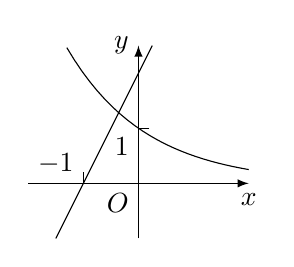
\begin{tikzpicture}[>=latex,scale=0.7]
\draw [->] (-2,0) -- (2,0) node [below] {$x$};
\draw [->] (0,-1) -- (0,2.5) node [left] {$y$};
\draw (0,0) node [below left] {$O$};
\draw [domain = -2:1.3] plot (-\x,{pow(2,\x)});
\draw (-1.5,-1) -- (0.25,2.5);
\draw (0.2,1) -- (0,1) node [below left] {$1$};
\draw (-1,0.2) -- (-1,0) node [above left] {$-1$};
\end{tikzpicture}}{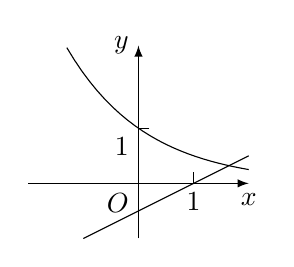
\begin{tikzpicture}[>=latex,scale=0.7]
\draw [->] (-2,0) -- (2,0) node [below] {$x$};
\draw [->] (0,-1) -- (0,2.5) node [left] {$y$};
\draw (0,0) node [below left] {$O$};
\draw [domain = -2:1.3] plot (-\x,{pow(2,\x)});
\draw (-1,-1) -- (2,0.5);
\draw (0.2,1) -- (0,1) node [below left] {$1$};
\draw (1,0.2) -- (1,0) node [below] {$1$};
\end{tikzpicture}}{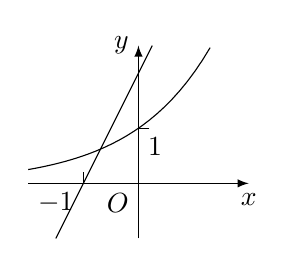
\begin{tikzpicture}[>=latex,scale=0.7]
\draw [->] (-2,0) -- (2,0) node [below] {$x$};
\draw [->] (0,-1) -- (0,2.5) node [left] {$y$};
\draw (0,0) node [below left] {$O$};
\draw [domain = -2:1.3] plot (\x,{pow(2,\x)});
\draw (-1.5,-1) -- (0.25,2.5);
\draw (0.2,1) -- (0,1) node [below right] {$1$};
\draw (-1,0.2) -- (-1,0) node [below left] {$-1$};
\end{tikzpicture}}{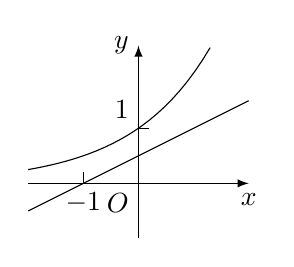
\begin{tikzpicture}[>=latex,scale=0.7]
\draw [->] (-2,0) -- (2,0) node [below] {$x$};
\draw [->] (0,-1) -- (0,2.5) node [left] {$y$};
\draw (0,0) node [below left] {$O$};
\draw [domain = -2:1.3] plot (\x,{pow(2,\x)});
\draw (-2,-0.5) -- (2,1.5);
\draw (0.2,1) -- (0,1) node [above left] {$1$};
\draw (-1,0.2) -- (-1,0) node [below] {$-1$};
\end{tikzpicture}}
\item 如图所示的是某池塘中的浮萍蔓延的面积$y$(单位: $\text{m}^2$)与时间$t$(单位: 月)的关系: $y=a^t$($a>0$且$a\ne 1)$. 
\begin{center}
\begin{tikzpicture}[>=latex,scale = 0.5]
\draw [->] (0,0) -- (4,0) node [below] {$t/\text{月}$};
\draw [->] (0,0) -- (0,9) node [left] {$y/\text{m}^2$};
\draw (0,0) node [below left] {$O$};
\draw [domain = 0:3.1] plot (\x,{pow(2,\x)});
\foreach \i in {1,2,3}{\draw [dashed] (\i,0) -- (\i,{pow(2,\i)}) -- (0,{pow(2,\i)}); \draw (\i,0) node [below] {$\i$};};
\foreach \i in {2,4,8}{\draw (0,\i) node [left] {$\i$};};
\end{tikzpicture}
\end{center}
以下结论:
\textcircled{1} 这个指数函数的底数是$2$; 
\textcircled{2} 第$5$个月时, 浮萍的面积就会超过$30\text{m}^2$;
\textcircled{3} 浮萍面积从$4\text{m}^2$到$12\text{m}^2$需要经过$1.5$个月;
\textcircled{4} 浮萍每个月增加的面积都相等. 其中, 正确结论的序号是\bracket{20}.
\fourch{\textcircled{1}\textcircled{2}\textcircled{3}}{\textcircled{1}\textcircled{2}\textcircled{3}\textcircled{4}}{\textcircled{2}\textcircled{3}\textcircled{4}}{\textcircled{1}\textcircled{2}}
\item 若$x>0$时, 指数函数$y=(a^2-1)^x$的值总大于$1$, 求实数$a$的取值范围.
\item 若$-1<x<0$, 比较$3^x, 3^{-x}$及$3^{2x}$的大小.
\item 设$a>1$, 若$a^{x^2+2x+1}<a^{2x^2-3x+1}$, 求实数$x$的取值范围.
\item 若函数$y=5^{x+1}+m$的图像不经过第二象限, 求实数$m$的取值范围. 
\item 求下列函数的定义域:\\
(1) $y=\log_a (x+12)$(常数$a>0$且$a\ne 1$);\\
(2) $y=\log_2\dfrac1{x^2-2x+5}$.
\item 已知对数函数$y=\log_ax$($a>0$且$a\ne 1)$的图像经过点$(3, 2)$. 若点$P(b, 4)$为此函数图像上的点, 求实数$b$的值.
\item 在同一平面直角坐标系中画出下列函数的图像, 并指出这些函数图像之间的关系.\\
(1) $y=\log_3x$;\\
(2) $y=\log_{\frac 13}x$;\\
(3) $y=(\dfrac 13)^x$.
\item 已知常数$a>0$且$a\ne 1$, 假设无论$a$取何值, 函数$y=\log_ax-1$的图像恒经过一个定点. 求此点的坐标.
\item 根据下列不等式, 确定底数$a$的取值范围:\\
(1) $\log_a 0.2<\log_a 0.1$;\\
(2) $\log_a\pi >\log_a\mathrm{e}$.
\item 已知$y=\log_{a^2-1}x$在区间$(0, +\infty)$上是严格减函数, 求实数$a$的取值范围.
\item 已知对数函数$y=\log_ax$($a>1$)在区间$[1, 2]$上的最大值比最小值大$1$, 求$a$的值.
\item 若$a>b>c>1$, 则下列不等式不成立的是\blank{50}. (填写所有不成立的不等式的序号)\\
\textcircled{1} $\log_ab>\log_ac$; \textcircled{2} $\log_a\dfrac 1b>\log_a\dfrac 1c$; \textcircled{3} $\log_{\frac 1a}b>\log_{\frac 1a}c$; \textcircled{4} $\log_{\frac 1a}\dfrac 1b>\log_{\frac 1a}\dfrac 1c$.
\item 设常数$a>0$且$a\ne 1$, 求函数$y=\log_a(a-a^x)$的定义域.
\item 根据下列不等式, 比较正数$m$及$n$的大小:\\
(1) $\log_3m<\log_3n$;\\
(2) $\log_am<\log_an$($a>0$且$a\ne 1$);\\
(3) $\log_mN<\log_nN$($0<m<1$, $0<n<1$, $0<N<1$).
\item 设$0<a<1$, 若$\log_a(4x^2-1)<\log_a(-2x^2+x+1)$, 求实数$x$的取值范围.
\item 比较$22^{23}$与$23^{22}$的大小.
\item 如果$^{237}\text{U}$在不断的裂变中, 每天所剩留质量与前一天剩留质量相比, 按同一比例减少, 且经过$7$天裂变, 剩余的质量是原来的$50\%$. 计算至少要经过多少天裂变, 其剩留质量才小于原来的$10\%$. 
\item 求下列函数的定义域:\\
(1) $y=\dfrac1{x^2+2x-3}$;\\
(2) $y=\sqrt{4-3x-x^2}$;\\
(3) $y=\sqrt{x-2}+\sqrt{x+3}$;\\
(4) $y=\dfrac 1{\lg(x+2)}+\dfrac 1{\sqrt{5-x}}$.
\item 设$p$、$q$是常数, 函数$y=f(x)$的表达式为$f(x)=x^2+px+q$. 若$f(1)=f(2)=0$, 求$f(-1)$.
\item 观察下列函数的图像, 并写出它们的值域:
\begin{center}
    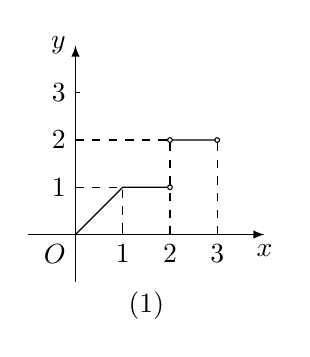
\begin{tikzpicture}[>=latex,scale = 0.6]
        \draw [->] (-1,0) -- (4,0) node [below] {$x$};
        \draw [->] (0,-1) -- (0,4) node [left] {$y$};
        \draw (0,0) node [below left] {$O$};
        \foreach \i in {1,2,3}
        {
          \draw (\i,0.1) -- (\i,0) node [below] {$\i$};
          \draw (0.1,\i) -- (0,\i) node [left] {$\i$};          
        };
        \draw (0,0) -- (1,1) -- (2,1) (2,2) -- (3,2);
        \draw [dashed] (0,1) -- (1,1) -- (1,0) (0,2) -- (2,2) (2,0) -- (2,2) (3,0) -- (3,2);
        \filldraw [fill = white, draw = black] (2,1) circle (0.05) (2,2) circle (0.05) (3,2) circle (0.05);
        \draw (1.5,-1) node [below] {(1)};
    \end{tikzpicture}
    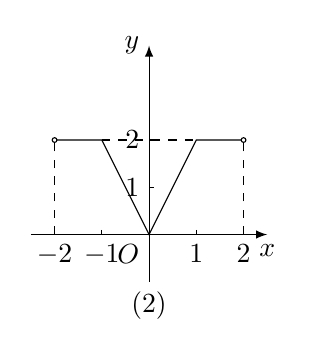
\begin{tikzpicture}[>=latex,scale = 0.6]
        \draw [->] (-2.5,0) -- (2.5,0) node [below] {$x$};
        \draw [->] (0,-1) -- (0,4) node [left] {$y$};
        \draw (0,0) node [below left] {$O$};
        \foreach \i in {1,2}
        {
          \draw (\i,0.1) -- (\i,0) node [below] {$\i$};
          \draw (0.1,\i) -- (0,\i) node [left] {$\i$};          
        };
        \foreach \i in {-1,-2}
        {
            \draw (\i,0.1) -- (\i,0) node [below] {$\i$};
        };
        \draw (-2,2) -- (-1,2) -- (0,0) -- (1,2) -- (2,2);
        \draw [dashed] (-2,0) -- (-2,2) (2,0) -- (2,2) (-1,2) -- (1,2);
        \filldraw [fill = white, draw = black] (-2,2) circle (0.05) (2,2) circle (0.05);
        \draw (0,-1) node [below] {(2)};
    \end{tikzpicture}
    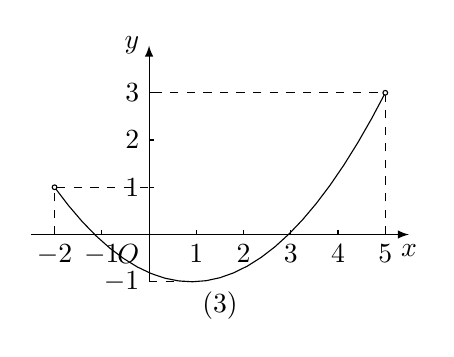
\begin{tikzpicture}[>=latex,scale = 0.6]
        \draw [->] (-2.5,0) -- (5.5,0) node [below] {$x$};
        \draw [->] (0,-1) -- (0,4) node [left] {$y$};
        \draw (0,0) node [below left] {$O$};
        \foreach \i in {-2,-1,1,2,3,4,5}
        {
            \draw (\i,0.1) -- (\i,0) node [below] {$\i$};
         
        };
        \foreach \i in {-1,1,2,3}
        {
            \draw (0.1,\i) -- (0,\i) node [left] {$\i$}; 
        };
        \draw [domain = -2:5] plot (\x,{2/49*(3+2*sqrt(2))*\x*\x+4/49*(-1-3*sqrt(2))*\x+(17-40*sqrt(2))/49});
        \draw [dashed] (0,-1) -- ({7*sqrt(2)-9},-1) (5,0) -- (5,3) -- (0,3) (-2,0) -- (-2,1) -- (0,1);
        \filldraw [fill = white, draw = black] (-2,1) circle (0.05) (5,3) circle (0.05);
        \draw (1.5,-1) node [below] {(3)};
    \end{tikzpicture}
\end{center}
\item 设$a$是常数, 求下列函数的定义域\\
(1) $y=\dfrac1{|x|-a}$;\\
(2) $y=\sqrt{x(x-a)}$.
\item 已知函数$y=f(x)$的表达式为$f(x)= \begin{cases} 2x(3+x), & x\ge 0,\\ 2x(3-x), & x<0.\end{cases}$ 求$f(2)$, $f(-4)$及$f(-a)$, 其中$a$为实数. 
\item 若函数$y=f(x)$的定义域为$\mathbf{R}$, 则$y=f(x)$为奇函数的一个充要条件为\bracket{20}.
\twoch{$f(0)=0$}{对任意$x\in \mathbf{R}$, $f(x)=0$都成立}{存在某个$x_0\in \mathbf{R}$, 使得$f(x_0)+f(-x_0)=0$}{对任意给定的$x\in \mathbf{R}$, $f(x)+f(-x)=0$都成立}
\item 证明下列函数$y=f(x)$为偶函数:\\
(1) $f(x)=x^2+x^{-2}$;\\
(2) $f(x)=\dfrac{x(2^x-1)}{2^x+1}$.
\item 证明下列函数$y=f(x)$为奇函数:\\
(1) $f(x)=x^{-3}$;\\
(2) $f(x)=\dfrac{\mathrm{e}^x-\mathrm{e}^{-x}}2$
\item 判断下列函数$y=f(x)$的奇偶性, 并说明理由:\\
(1) $f(x)=2x+\sqrt[3]x$;\\
(2) $f(x)=2x^4-x^2$;\\
(3) $f(x)=x^2-x$;\\
(4) $f(x)=\dfrac{1-x}{1+x}$;\\
(5) $f(x)=\lg\dfrac {1-x}{1+x}$.
\item 证明:函数$y=x-\dfrac 1x$, $x\in (-\infty, 0)$是严格增函数.
\item 证明:函数$y=\lg (1-x)$在其定义域上是严格减函数.
\item 求下列函数的最大值与最小值, 并写出取最值时相应自变量的值:\\
(1) $y=x^2-4x-2$;\\
(2) $y=6x-3x^2$;\\
(3) $y=-x^2-4x-3$, $x\in [-3, 1]$;\\
(4) $y=x^2-2x-3$, $x\in [-2, 0]$.
\item 求函数$y=\log_{\frac 12}(x+2)$, $x\in [2, 6]$的最大值与最小值.
\item 已知$y=x^2+px+q$和$y=x+\dfrac 4x$都是定义在$[1, 4]$上的函数, 且在$x_0$处同时取到相同的最小值. 求$y=x^2+px+q$的最大值.
\item 已知实数$b<2$, 而函数$y=x^2+ax+1$, $x\in [b, 2]$是偶函数. 求实数$a$、$b$的值.
\item 判断下列函数$y=f(x)$的奇偶性, 并说明理由:\\
(1) $f(x)=\dfrac{10^x-10^{-x}}{10^x+10^{-x}}$;\\
(2) $f(x)=x(\dfrac 1{2^x-1}+\dfrac 12)$.
\item 当表达式$f(x)=$\blank{50}时, 函数$y=f(x)$同时满足以下条件:\\
\textcircled{1} 不是偶函数;\\
\textcircled{2} 在区间$(-\infty, -1)$上是严格减函数;\\
\textcircled{3} 在区间$(0, 1)$上是严格增函数.
\item 作出函数$y=x^2-2|x|$的大致图像, 并分别写出它的定义域、奇偶性、单调区间及最小值.
\item 研究函数$y=\dfrac1{1+x^2}$的定义域、奇偶性、单调性及最大值.
\item 如果函数$y=x^2-2mx+1$在区间$(-\infty, 2]$上是严格减函数, 那么实数$m$的取值范围为\blank{50}.
\item 设$t$是实数, 且$t<4$. 求函数$y=|2^{x+1}-8|$, $x\in [t, 4]$的最小值.
\item 某企业去年四个季度生产某种型号机器的数量$y$(单位:万台)与季度$x$的函数关系如下表所示:
\begin{center}
\begin{tabular}{|c|c|c|c|c|}
\hline
$x$/季度 & $1$ & $2$ & $3$ & $4$ \\ \hline
$y$/万台 & $10$ & $12$ & $14$ & $16$ \\ \hline
\end{tabular}
\end{center}
试写出该函数的定义域, 并作出其大致图像.
\item 某地区住宅电话费收取标准为: 接通后$3$分钟内(含$3$分钟)收费$0.20$元, 以后每分钟(不足$1$分钟按$1$分钟计)收费$0.10$元. 如果一次通话时间为$t$(单位: $\text{min}$), 写出通话费$y$(单位: 元)关于通话时间$t$的函数关系.
\item 求函数$y=\sqrt{2x+1}-x+1$的零点.
\item 已知函数$y=x^3+x^2+x-1$在区间$(0, 1)$上有且仅有一个零点, 用二分法求该零点的近似值. (结果精确到$0.1$)
\item 已知某气垫船的最大船速是$48$海里/时, 船每小时使用的燃料费用和船速的平方成正比. 当船速为$30$海里/时时, 船每小时的燃料费用为$600$元, 而其余费用(不论船速为多少)都是每小时$864$元. 船从甲地行驶到乙地, 甲乙两地相距$100$海里.\\
(1) 试把船每小时使用的燃料费用$P($单位: 元)表示成船速狏(单位: 海里/时)的函数;\\
(2) 试把船从甲地到乙地所需的总费用$y$(单位:元)表示成船速$v$(单位: 海里/时)的函数;\\
(3) 当船速为多少时, 船从甲地到乙地所需的总费用最少?
\item 为分流短途乘客, 减缓轨道交通高峰压力, 某地地铁实行新的计费标准, 其分段计费规则如下: $0$至$6\text{km}$(含$6\text{km}$)票价$3$元; $6$至$16\text{km}$(含$16\text{km}$)票价$4$元; $16\text{km}$以上每$6\text{km}$(不足$6\text{km}$时按$6\text{km}$计)票价递增$1$元, 但总票价不超过$8$元.\\
(1) 试作出票价$y$(单位: 元)关于路程$x$(单位: $\text{km}$)的函数的大致图像;\\
(2) 某人买了$5$元的车票, 他乘车的路程不能超过多少?
\item 某物流公司在上海及杭州的仓库分别有某机器$12$台和$6$台, 现决定销售给$A$市$10$台、$B$市$8$台. 已知上海调运一台机器到$A$、$B$市的运费分别为$400$元和$800$元; 杭州调运一台机器到$A$、$B$市的运费分别为$300$元和$500$元. 设从上海调运$x$台机器往$A$市, 求总运费$y$(单位: 元)关于$x$(单位: 台)的函数关系.
\item 证明: 方程$\lg x+2x=16$没有整数解.
\item 解不等式: $\dfrac 2{x^2}\ge 3x-1$. 
\item 已知函数$y=x^2-4x-5$, $x\in [1, 3]$, 判断其是否存在反函数. 若存在, 求出反函数; 若不存在, 说明理由.
\item 求下列函数的反函数:\\
(1) $y=-x^3$;\\
(2) $y=\dfrac x{x+2}$;\\
(3) $y=x^2+1$, $x\in (-\infty, 0)$.
\item 求下列函数的反函数:\\
(1) $y=10^x+1$;\\
(2) $y=\log_2(x+1)$;\\
(3) $y=\log_2(2x)$.
\item 已知$f(x)=1-\log_2x$, 设$y=f^{-1}(x)$是$y=f(x)$的反函数. 求$f^{-1}(-3)$的值.
\item 已知函数$y=\dfrac a{x+1}$的反函数的图像经过点$(\dfrac 12, 1)$, 求实数$a$的值.


\end{enumerate}

\end{document}